\documentclass{article}
\usepackage{graphicx}
\usepackage{hyperref}

\begin{document}
\section{Introduction}
GFS is a scalable distributed file system for large distributed data-intensive
applications. It provides fault tolerance while running on inexpensive
commodity hardware, and it delivers high aggregate performance to a large
number of clients. Large deployments of GFS are capable of providing hundreds
of terabytes of storage across thousands of disks on over a thousand machines,
and it is concurrently accessed by hundreds of clients.

First, component failures are the norm rather than the
exception. The file system consists of hundreds or even
thousands of storage machines built from inexpensive commodity parts and is accessed by a comparable number of
client machines. The quantity and quality of the components virtually guarantee that some are not functional at
any given time and some will not recover from their current failures. We have seen problems caused by application
bugs, operating system bugs, human errors, and the failures
of disks, memory, connectors, networking, and power supplies. Therefore, constant monitoring, error detection, fault
tolerance, and automatic recovery must be integral to the
system.

Second, files are huge by traditional standards. Multi-GB
files are common. Each file typically contains many application objects such as web documents. When we are regularly
working with fast growing data sets of many TBs comprising
billions of objects, it is unwieldy to manage billions of approximately KB-sized files even when the file system could
support it. As a result, design assumptions and parameters
such as I/O operation and blocksizes have to be revisited

Third, most files are mutated by appending new data rather than overwriting
existing data. Random writes within a file are practically non-existent. Once
written, the files are only read, and often only sequentially. A variety of
data share these characteristics. Some may constitute large repositories that
data analysis programs scan through. Some may be data streams continuously
generated by running applications. Some may be archival data. Some may be
intermediate results produced on one machine and processed on another, whether
simultaneously or later in time. Given this access pattern on huge files,
appending becomes the focus of performance optimization and atomicity
guarantees, while caching data blocks in the client loses its appeal.

Fourth, co-designing the applications and the file system API benefits the
overall system by increasing our flexibility.  For example, we have relaxed
GFS’s consistency model to vastly simplify the file system without imposing an
onerous burden on the applications. We have also introduced an atomic append
operation so that multiple clients can append concurrently to a file without
extra synchronization between them. 

 \section{Interface}
 GFS provides a familiar file system interface, but not POSIX semantics.
 Files are organized hierarchically in directories
 and identified by pathnames. The operations \texttt{create},
 \texttt{delete}, \texttt{open}, \texttt{close}, \texttt{read}, \texttt{write},
 and most interestingly, \texttt{append} to files is provided.

\section{Architecture}

\begin{figure}
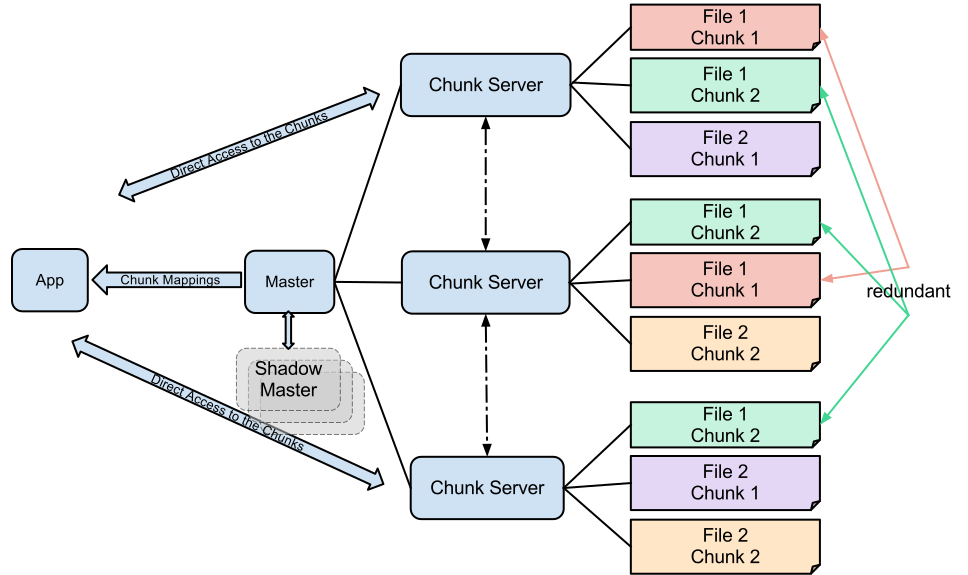
\includegraphics[width=\textwidth]{gfs-diagram.pdf}
\caption{GFS architecture}
\label{fig:architecture}
\end{figure}

On the server-side, there is a single \emph{master} controlling multiple slaves,
known as \emph{chunkservers}. These are accessed by multiple clients, as
shown in  Figure \ref{fig:architecture}.

The single master maintains all metadata. The metadata includes access control,
mapping files to chunks, and mapping of chunks to the chunkservers which
contain them.  The presence of a single master allows GFS to sidestep complex
logic around multiple-sources-of-truth. 

Files are divided into fixed-size \emph{chunks}. Each chunk is identified by an
immutable and globally unique 64 bit chunk handle assigned by the master at the
time of chunk creation.  Chunkservers store chunks on local disks as Linux files
and read or write chunk data specified by a chunk handle and offset. For
reliability, each chunk gets replicated on multiple chunkservers. The user
can modify the number of replicas stored; the default is 3. The master
periodically communicates with each chunkserver in HeartBeat messages to give
it instructions and collect its state.


Clients interact with the master for metadata operations, but all data-bearing
communication goes directly to the chunkservers. This prevents bottlenecking
the master; within GFS, lightweight control flow occurs by communication with
the master; heavyweight dataflow is performed by directly talking to the
chunk servers.

\section{Master Design}

We describe the design of the master in detail. In GFS, there
is a \emph{single master} at any given moment. Being a single leader, the
master can take sophisticated chunk placement and replication decisions using
global knowledge. 

The sequence of events for a client to fetch a file from GFS is:
\begin{itemize}
    \item[1]  The client wishes to read data from a file $f$ starting from byte offset $o$, of
        some length $l$. using the fixed chunk size, the client translates the
        byte offset into a chunk index ($b/\texttt{chunksize}$) within the file.
        It sends the request of (file, chunk index) to the master.
    \item[2]  The master replies with the corresponding chunk handle and
        locations of the replicas \emph{(control-flow)}.
    \item[3] The client caches this information using the file name and
        chunkindex as the key.
    \item[4] The client then sends a request to one of the replicas.
        The request specifies the chunk handle and a byte range within that
        chunk. \emph{(data-flow)}.
    \item[5] Further reads of the same chunk require no more client-master
        interaction.
\end{itemize}

\subsection{Data Owned By Master}
The master stores three major types of metadata: the file and chunk
namespaces, the mapping from files to chunks, and the locations of each chunk’s
replicas.

All metadata is kept \textbf{in-memory}. The first two types (namespaces
and file-to-chunkmapping) are also kept persistent by logging mutations to an
operation log stored on the master’s local disk, and replicated on remote
machines. Using a log allows us the master state to be updated simply, reliably,
and without risking inconsistencies in the event of a master crash. 

The master does not store chunk location information persistently. Instead, it
asks each chunkserver about its chunks at master startup and whenever a
chunkserver joins the cluster.  Since metadata is stored in memory, master
operations are fast. Furthermore, it is easy and efficient for the master to
periodically scan through its entire state in the background. The master does
not keep a persistent record of which chunkservers have a replica of a given
chunk. It simply polls chunkservers for that information at startup. The master
can keep itself up-to-date thereafter because it controls all chunkplacement
and monitors chunkserver status with regular HeartBeat message.

\subsection{The Master Operation Log}

The operation log contains a historical record of critical metadata changes.
It is a persistent record of metadata; it also serves as a logical time line 
that defines the order of concurrent operations. 

Files, chunks, and their versions are all uniquely and eternally identified by
the logical times at which they were created.  Since the operation log is
critical, It must be stored reliably. Otherwise, one can  effectively lose the
whole file system or recent client operations even if the chunks themselves
survive, due to a loss of metadata of which chunk does what.  Therefore, the
operation log is replicated on multiple remote machines; client operations are
responded to only after flushing the corresponding log record to disk both
locally and remotely.

The master recovers its file system state by
replaying the operation log. To minimize startup time, the log is kept small
through the use of checkpointing. The master checkpoints its state whenever
the log grows beyond a certain size; this allows fast recovery by loading the
latest checkpoint from local disk and replaying only the limited number of log
records after that. A failure during checkpointing does not affect correctness
because the recovery code detects and skips incomplete checkpoints.

\subsection{Namespacing And Locking}

Many master operations can take a long time. We do not want to delay other
master operations for one expensive operation. Therefore, we allow multiple
operations to be active and use locks over regions of the namespace to ensure
proper serialization.


Unlike traditional file systems, GFS does not have a per-directory data
structure that lists all the files in that directory (ie, the \texttt{inode}).
Nor does it support aliases for the same file or directory (i.e, hard or
symbolic links). GFS logically represents its namespace as a lookup table
mapping full pathnames to metadata. With a trie-like data structure for
compression, this table can be efficiently represented in memory. Each node
in the namespace tree (both absolute file names and
absolute directory names) have an associated read-write lock.
Each master operation acquires a set of locks before it
runs. Typically, if it involves \texttt{/d1/d2/.../dn/leaf}, it will
acquire read-locks on the directory names \texttt{/d1}, \texttt{/d1/d2, ...},
\texttt{/d1/d2/.../dn}, and either a read lock or a write lock on the
leaf node \texttt{/d1/d2/.../dn/leaf}. Note that leaf may be
a file or directory depending on the operation.


Consider an exaple of how this locking mechanism can prevent a file
\texttt{/home/user/foo} from being created while \texttt{/home/user} is being
snapshotted to /save/user. The snapshot operation acquires read lock on 
\texttt{/home} and \texttt{/save}, and write locks on \texttt{/home/user} and 
\texttt{/save/user}. The file creation
acquires read locks on \texttt{/home} and \texttt{/home/user}, and a write lock
on \texttt{/home/user/foo}.
The two operations will be serialized properly because they try to obtain
conflicting locks on \texttt{/home/user}. 

File creation does not require a write lock on the parent directory because
there is no 'directory'/ \texttt{inode} data structure to be protected from
modification.  The read lock on the name is sufficient to protect the parent
directory from deletion.

\section{Client operations}

\subsection{Reads}

\subsection{Mutations: Writes And Appends}

A mutation is an operation that changes the contents or metadata of a chunk
such as a write or an append operation. Each mutation is performed at all the
chunk’s replicas. Leases are used to maintain a consistent mutation order across
replicas. The master grants a chunk lease to one of the replicas, which we call
the \textbf{primary replica for that chunk}. The primary picks a serial order for all mutations to the chunk.
All replicas follow this order when applying mutations. 

The lease mechanism is designed to minimize management overhead at the master.
A lease has an initial timeout of 60 seconds. However, as long as the chunk 
is being mutated, the primary receive extensions from the master indefinitely.
These extension requests and grants are piggybacked on the HeartBeat messages
regularly exchanged between the master and all chunkservers.  The master may
sometimes try to revoke a lease before it expires (e.g., when the master wants
to disable mutations on a file that is being renamed). Even if the master loses
communication with a primary, it can safely grant a new lease to another
replica after the old lease expires.

The sequence of events from a client's perspective to perform a write
are as follows:

\begin{itemize}
\item[1] The client asks the master which chunkserver holds the current lease
    for the chunk, and the locations of the other replicas. If no one has a
        lease, the master grants a lease to some replica.


\item[2] The master replies with the identity of the primary and the
    locations of the secondary replicas. The client caches this data
    for future mutations. The client contacts the master again only when
    the primary becomes unreachable or replies that it no longer holds a
    lease. 

\item[3] The client pushes the data to all the replicas. A client can do so in
    any order. This data is stored in a buffer in the replica; it is 
        emph{not yet written}.

\item[4] Once all the replicas have acknowledged receiving the data, the client
    sends a write request to the primary. The request identifies the data
        pushed earlier to all of the replicas. The primary assigns consecutive
        serial numbers to all the mutations it receives, possibly from multiple
        clients, which provides the necessary serialization. It applies the
        mutation to its own local state in serial number order.

\item[5] The primary forwards the write request to all secondary replicas. Each
    secondary replica applies mutations in the same serial number order
    assigned by the primary.

\item[6] The secondaries all reply to the primary indicating that they have
    completed the operation.

\item[7] The primary replies to the client. Any errors encountered at any of
    the replicas are reported to the client.  In case of errors, the write may
        have succeeded at the primary and an arbitrary subset of the secondary
        replicas. (If it had failed at the primary, it would not have been
        assigned a serial number and forwarded.) The client request is
        considered to have failed, and the modified region is left in an
        inconsistent state. It is the responsibility of the client
        to handle such failures by retrying steps (3) through (7).
\end{itemize}


\subsection{Special support for \texttt{append}s}

Record append is heavily used to model many-producer-queues.

In a traditional write, the client specifies the offset at which data is to be
written. Concurrent writes to the same region are not serializable: the region
may end up containing data fragments from multiple clients. In a record append,
however, the client specifies only the data. GFS appends it to the file at
least once atomically (i.e., as one continuous sequence of bytes) at an offset
of GFS’s choosing and returns that offset to the client. 

If a record append fails at any replica, the client retries the operation. As a
result, replicas of the same chunk may contain different data possibly including
duplicates of the same record in whole or in part. GFS does not guarantee that
all replicas are bytewise identical. It only guarantees that the data is
written at least once as an atomic unit. 

\subsection{Snapshot}

The snapshot operation makes a copy of a file or a directory tree (the
“source”) almost instantaneously, while minimizing any interruptions of ongoing
mutations. This can be used to branch copies of huge data sets
(and often copies of those copies, recursively), or to checkpoint the current
state before experimenting with changes that can later be committed or rolled
back. Copy-on-write is used to implement snapshots. 

When the master receives a snapshot request, it first
revokes any outstanding leases on the chunks in the files it is about to
snapshot. This ensures that any subsequent writes to these chunks will require
an interaction with the master to find the lease holder. This will give the
master an opportunity to create a new copy of the chunk first. 

After the leases have been revoked or have expired, the master logs the
operation to disk. It then applies this log record to its in-memory state by
duplicating the metadata for the source file or directory tree. The newly
created snapshot files point to the same chunks as the source files.  The first
time a client wants to write to a chunk \texttt{C} after the snapshot operation, it sends
a request to the master to find the current lease holder. The master notices
that the reference count for chunk \texttt{C} is greater than one. It defers replying to
the client request and instead picks a new chunk handle \texttt{C’}. 
It then asks each chunkserver that has a current replica of \texttt{C} to create a new
chunk called \texttt{C’}. By creating the new chunk on the same chunkservers as the
original, the data can be copied locally, not over the
network.  From this point, request handling is no different from that for any chunk: the
master grants one of the replicas a lease on the new chunk \texttt{C’} and
replies to the client, which can write the chunk normally, not knowing that it
has just been created from an existing chunk.

\bibliographystyle{plain}
\bibliography{references}
\nocite{*}
\end{document}
